\documentclass[sigplan,10pt,review]{acmart}
\settopmatter{printfolios=true,printccs=false,printacmref=false}


\usepackage{inputenc}
\usepackage{amsmath}
\usepackage{graphicx}
\usepackage{float}
\usepackage{geometry}

\setcopyright{acmcopyright}
\copyrightyear{2022}
\acmYear{2022}
\acmDOI{}


\acmConference[COMP 764]{XYZ}{Winter 2022}{Montreal, Quebec, Canada}

\acmBooktitle{Yay book} 
\acmPrice{Free}
\acmISBN{}

\title{Constraint driven Scheduling of fine-grained C concurrency for Reconfigurable Hardware}
\author{Akshay Gopalakrishnan}
\affiliation{McGill University}
\email{akshay.akshay@mail.mcgill.ca}
\date{today}

\begin{document}

    \maketitle 

    %Introduction to the course project 

\section{Introduction}

    The recent decades have seen the growing utilization of specialized hardware for the purpose of extensive computing. 
    Right from general purpose CPUs to highly specialized hardware such as ASICs are being used in a wide variety of applications.
    When it comes to specialized hardwares there is an increasing usage of FPGAs especially due to its advantage of reprogrammability as per user's need.
    In this endeavor, to synthesize such FPGA, high level synthesis(HLS) tools have been introduced.
    HLS is a process of High Level Synthesis(HLS) is a process of mapping behavioral(C-like programs) models of hardware to low level(HDL-like programs) ones; which are then synthesized as specialized hardwares(eg: FPGA, ASIC). 
    HLS tools are used widespread in recent times due to the high demand for such specialized hardware than have better throughput and energy consumption for specific intensive computations(eg: in Machine Learning).

    However, HLS has been predominantly used/developed for sequential programs. 
    The last few years have been investigated in terms of synthesizing concurrent programs; how would specialized hardware be synthesized that reflects concurrency.
    However, not much investigation has been done when it comes to synthesis of fine-grained concurrent programs; commonly known as lock-free programs.



    %Related work

\section{Related Work}

    %Start with HLS tools
    Several HLS tools are available today; some of the notables being Quartus and LegUp. 
    LegUp allows their users to insert behavioral models of hardware in C language. 
    Several works were done further to extend LegUp in synthesizing concurrent C programs to hardware.  
    
    \cite{DBLP:conf/fpt/ChoiBA13} propose a method to map software threads to parallel hardware for FPGAs. 
    They do this for programs that utilize pthreads and OpenMP constructs.
    However, their focus was mainly on lock-based concurrency in C. 
    They do note in their experiments that having a constraint on resources to map threads does effect the schedule(more cycles). 
    Their contributions were integrated into LegUp.

    \cite{DBLP:conf/fpga/RamanathanFWC17} investigate the synthesis of concurrent programs utilizing fine grained concurrency elements of C.
    They show that on using atomics primitives provided by C, incorrect schedules can be obtained.
    They remedy this by adding additional ordering constraints among memory accesses.
    They test their approach by extending LegUp to tackle fine grained concurrent constructs of C.
    \cite{DBLP:journals/tc/RamanathanWC18} is a follow up to this work implementing pipelined scheduling for such programs.
        
    %Put optimization thing here
    When it comes to HLS tools, one major advantage is the optimizations we can do at the behavioral model itself. 
    These optimizations, have also been proven to significantly improve the resultant hardware synthesized.
    \cite{DBLP:conf/lcpc/CongLPZ12} and \cite{DBLP:conf/fccm/HuangLCCXBA13} show the impact/effect of compiler optimizations on HLS for Reconfigurable hardware like FPGAs.
    Specifically, they show how scheduling(termed as latency) has a major impact due the optimization passes of the compiler, as well as the order in which we perform it. 
    But their work does not address this impact on concurrent programs(let alone those using fine grained Concurrency) synthesized to hardware. 

    While we do want to perform aggressive optimizations for concurrent behavioral models, we are constrained by the semantics of such programs.
    \cite{DBLP:conf/popl/VafeiadisBCMN15} shows that programs utilizing fine grained concurrency of C do not get the benefit of some optimizations as they are rendered unsafe in a concurrent context. 
    \cite{DBLP:conf/fccm/RamanathanCW18} try to identify which memory accesses can be safely reordered in a weakly consistent C program targeted for hardware synthesis.
    Their goal was to improve the overall schedule of the program, and in turn the hardware that is synthesized for it. 
    \cite{DBLP:journals/tvlsi/RamanathanCW21} is a follow up to this work describing a global analysis to more aggressively perform safe reorderings of memory accesses for the same purpose.

    Previous works in the line of synthesizing weakly consistent C programs assume that every thread can be mapped to a unique hardware accelerator during synthesis. 
    They do not investigate the effect of constraining the number of available accelerators.
    While reordering was proposed in this line to improve schedules, no investigation was done on whether any optimization could have an impact on number of resources required for synthesis. 
    Moreover, minimization of resources was not a factor considered in this effort; as the primary goal was to get overall correct schedule; and doing optimizations to help lower the required clock cycles. 




    %Show why optimizations can be effective for better synthesis
    %Show work that investigates on synthesizing concurrent C programs to FPGA
    %Show work that investigates syntehsizes fine grained concurrent C programs 
    %Showcase the limitations for each of them
    

    \section{Methodology}

    Previous work on synthesizing fine grained concurrent programs assumed infinte resources (hardware accelerators).
    In practice this is not true. 
    One straightforward direction is to consider a more global scheduling approach to reuse resources.
    However, coming up with a sound global analysis that respects all consistency rules of the concurrency model might be non-trivial task.
    Instead, I propose to address the resource constraint problem by performing an optimization that merges two or more threads.
    Previous work has shown that optimizations do significantly improve the resource requirements. 
    However, the optimizations considered were only for sequential programs; while merging two threads is something for concurrent programs. 
    Hence, we investigate whether this optimization indeed helps our case.

    The main goal is to identify if we can minimize resource utilization while performing synthesis of concurrent programs such as above.
    We assume from previous work that synthesis is done per-thread; each thread is scheduled independently and allocated its own share of resources.
    In this endeavor, I have only addressed the correct scheduling and performing this optimization at the pre-scheduling stage.
    I do not implement the full HLS process; the program; if concurrent, cannot be synthesized into VHDL as of now. 

    %Explain here what you exactly need 
    \subsection{Concurrency Model}

        There are several shared memory concurrency models that exist to date.
        Previous work has mainly focused on C based concurrency.
        The C concurrency model semantics is fairly non-trivial to tackle as well as implement. 
        Hence, I choose a standard intuitive model widely understood; Sequential Consistency\cite{Lamport79}. 

    \subsection{Types of Programs}

        The programs are considered to be a set of statements of the following format 
        \begin{align}
            a \ = \ b \ + \ cs
        \end{align}
        Here $a$ refers to some memory.
        $b$ and $cs$ can be either memory or constants. 

        Memory can be termed as local ($a$ and $b$) or global/shared ($cs$ - any memory name ending with $s$).

        Each program is viewed as a set of threads; each of which have the following statements as above. 
        There are no coniditional branching statements, nor loops. 
        
    \subsection{Code Base Utilized}

        For the implementation, I reuse the existing code base from Assignment. 
        The assignment dealt only with sequenital programs of the above form. 
        The extension thus, must be done to incorporate concurrency reflecting SC.

    \subsection{Additions to Code base}
    
        \paragraph*{Threads}
            The notion of threads is easily captured by the code-base by representing each thread as its own DFG. 
            
        \paragraph*{Correct Scheduling}

            One important thing to address is that of ensuring correct scheduling in a concurrent context.
            \cite{DBLP:conf/fpga/RamanathanFWC17} showed that without adding extra memory dependencies, one can get an incorrect schedule for synthesis. 
            Thus, the solution was to add additional dependencies between memory accesses which are shared. 
            For sequential consistency, the dependencies were identified to be between every shared memory access in the same thread.
            Fig~\ref{scord} represents the following functions that were created for this
            \begin{figure}
                \centering
                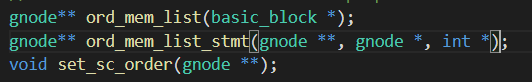
\includegraphics[scale=0.5]{Sc-order.PNG}
                \caption{Three functions created to take a thread and add additional memory dependencies respecting Sequential Consistency.}
                \label{scord}
            \end{figure}

            Adding these dependency edges, the scheduler must also incorporate this information while alloting an action to a specific clock cycle time stamp. 
            Fig~\ref{Schd} showcases the code snippet that was added for this. 
            Note that because we still use the previous approach of independently scheduling each thread, these changes were identified to be sufficient for correct scheduling. 
            \begin{figure}
                \centering
                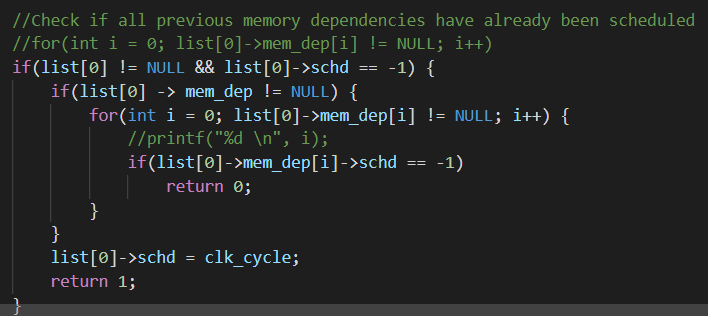
\includegraphics[scale=0.5]{Schd.PNG}
                \caption{Code snippet added to factor in memory dependencies while scheduling}
                \label{Schd}
            \end{figure}

        \paragraph*{Merging Optimization}
    
        I have implemented a DFG as a set of DFGs in my code base.
        Thus, merging was equivalent to simply adding one DFG into another. 
        While merging, memory dependencies that are newly introduced must also be taken care of.
        This differentiates the different merging combinations.
        Since the DFG set is implemented as an array of DFGs, the implicit array order was used to retain the memory order after merging.
 
        Fig~\ref{merge} represents the above idea. 
        Here $t1$ and $t2$ are two threads which are a set of DFGs. 
        $merge$ is the new program that is to be constructed using the elements of $t1$ and $t2$. 
        \begin{figure}
            \centering
            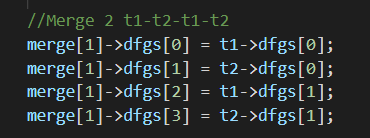
\includegraphics[scale=0.5]{Merge.PNG}
            \caption{Merging is equivalent to just adding and mixing DFG components of one thread with another}
            \label{merge}
        \end{figure}

        %Insert code snippet

    \paragraph*{Soundness?}

        An important factor to consider is whether such merging is a sound Transformation. 
        \cite{DBLP:journals/pcs/MoiseenkoPK21}, in their survey paper, do however, mention merging as a sound transformation under Sequential Consistency (SC).
        So a formal proof is not required.
 
    %Explain how you combine all of them into one specific total order on memory events

    %Show code snippets that you inserted for them in your existed code base

    %Showcase why this works (sketch proof?)

    
\section{Experimental Setup}

    %Explain your program purpose
    I specifically wanted to capture different program patterns that captures the following features
    \begin{itemize}
        \item Captures Read-Write, Read-Read, Write-Read, Write-Write dependencies between shared memory.
        \item Logical resources (adders) used by such programs.
        \item Mixture of shared and local memory usage.
    \end{itemize}

    Since I assume my programs have no conditionals or loops, I wanted to capture relatively general program patterns that may possibly occur while performing optimizations. 
    To capture all the above features, the following program format deemed sufficient as that in Fig~\ref{P1}.
    \begin{figure}[H]
        \centering
        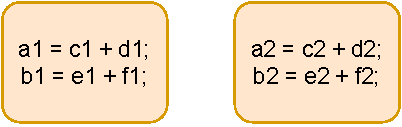
\includegraphics[scale=0.5]{Prog.pdf}
        \caption{Program Format}
        \label{P1}
    \end{figure}

    For each of the above accesses, I create a program where either they are shared or not. 
    For example, $a1$ can be either just $a1$ or $as$ (in this way, I capture the notion of shared memory between the two threads, since $a2$ may also become $as$.)
    This way, in total, I get 4096 programs. 

    %How it represents the patterns the compiler optimization would have 

    %Show how it covers the MP, SB, LB ordering patterns 

    %Show how it covers the resource constraint problem 

    %Detail the stats (how maby programs, how many sharred accesses, etc)

    \section{Evaluation}

    %Showcase the graph that summarizes the approach (scatter plot for different merge strategies)
    The above programs were run and tested for each merging strategy. 
    On merging, they were measured for the following: 
    \begin{itemize}
        \item Clock cycles utilized after merging. 
        \item Max resources that we require after merging. 
    \end{itemize}

    I also measured before merging, for each program, the clock cycles and adders required for each thread. 
    It is important to note that the total clock cycles represent the worst case scenario; if this program was run without merging. 

    The overall result was positive; it was possible to reduce or maintain the number of resources required, in addition to reducing the worst case number of clock cycles.
    Fig~\ref{Fig1} showcases the clock cycles saved from the worst case on merging: 
    %Insert graph here 
    \begin{figure}
        \centering
        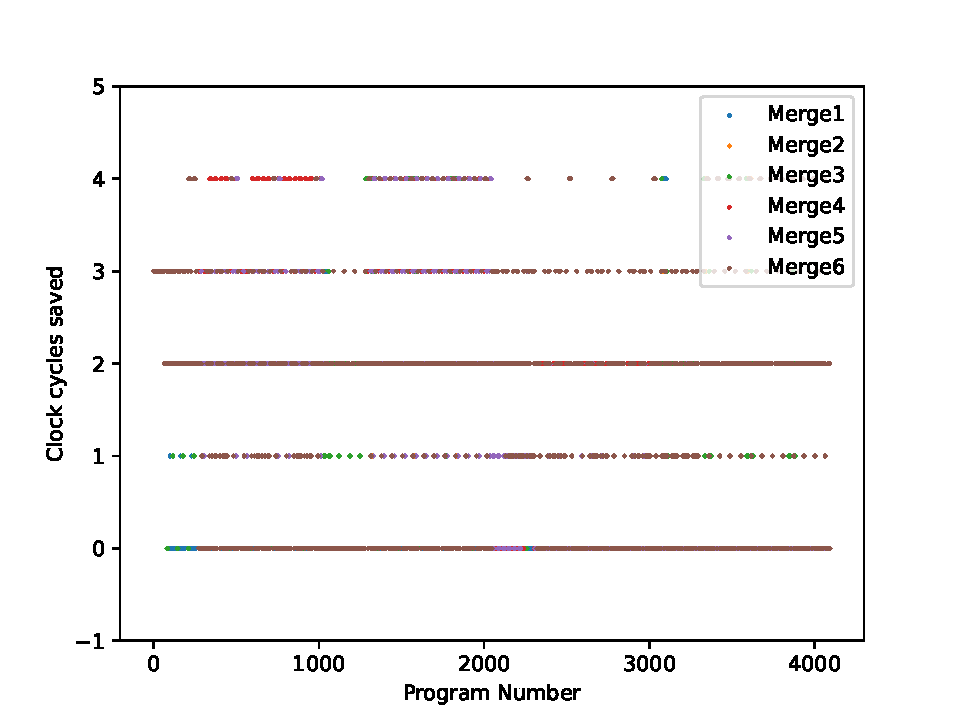
\includegraphics[scale=0.5]{m01.pdf}
        \caption{Scatter plot for each merging strategy, showing how many clock cyces were saved}
        \label{Fig1}
    \end{figure}

    I noticed that for each program, the clock cycles saved is at least zero.
    This shows us that at least merging does not result in total clock cycles required to be more than the original program. 
    The reason for this is quite intuitive; merging is equivalent to saying one thread executes first, followed by the second.
    Hence, naturally, the clock cycles will be bounded by the worst case before merging. 

    What is interesting however, is that the clock cycles are better than the worst case in almost 70percent of the programs that were considered after merging. 
    Fig~\ref{Fig2} shows the count of programs where (irrespective of how we merge) we save clock cycles on merge.  
    
        %inser graph here of clk_count 
        \begin{figure}
            \centering
            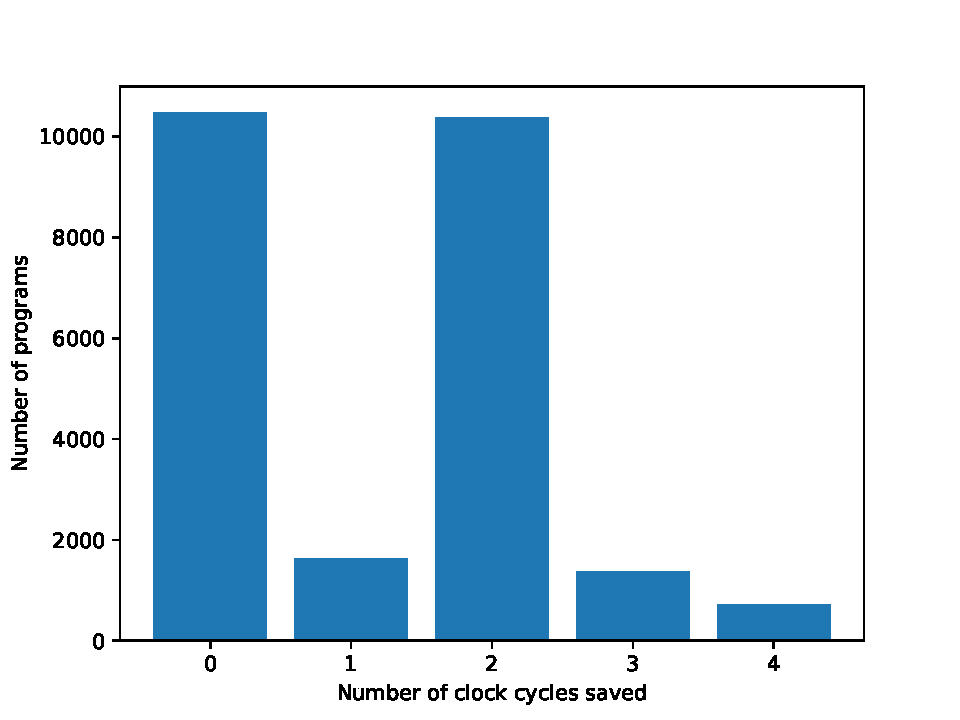
\includegraphics[scale=0.5]{clk_count.pdf}
            \caption{Count of programs after merging for the number of clock cycles saved.}
            \label{Fig2}
        \end{figure}
    
    
    This shows us a promise that merging indeed may not be detrimental to number of clock cycles; there will exist some merging that helps us save clock cycles in most cases.

    When it comes to resources, Fig~\ref{Fig3} showcases the resources saved (in comparison to pre-merge the amount of resources required).
    I noticed with the scatter plot that, once again, the amount of resources required is bounded by the amount required pre-merge. 
    What is interesting however, is that resources are saved, even though the scheduling algorithm is greedy, assuming infinte resources.
    This occured as adding additional memory dependency edges implicitly added dependency edges between the addition action too (this occurs due to Read-Write or Write-Read dependency edges). 
    \begin{figure}
        \centering
        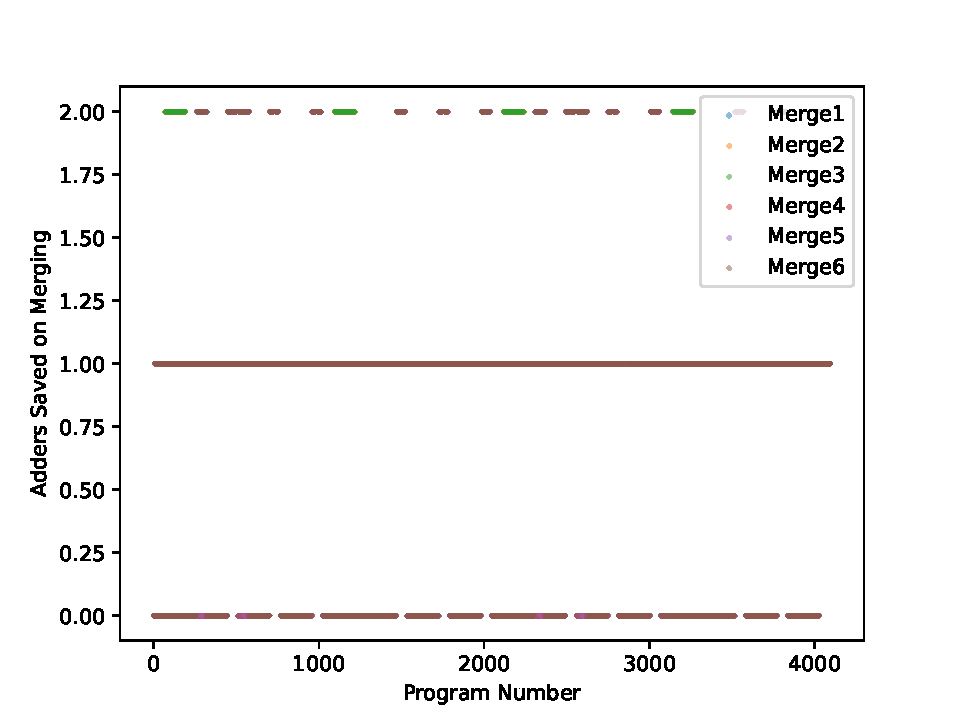
\includegraphics[scale=0.5]{m02.pdf}
        \caption{Scatter plot for each merging strategy, showing how many adders were saved}
        \label{Fig3}
    \end{figure}
    
    Fig~\ref{Fig4} shows us the count of programs (irrespective of how we merge) for the amount of resources we saved on merging.
    Once again, for most cases, some form of merging saved resources. 
    This is promising; as this shows us that resource constraints can be addressed by an optimization which just merges threads. 
    \begin{figure}
        \centering
        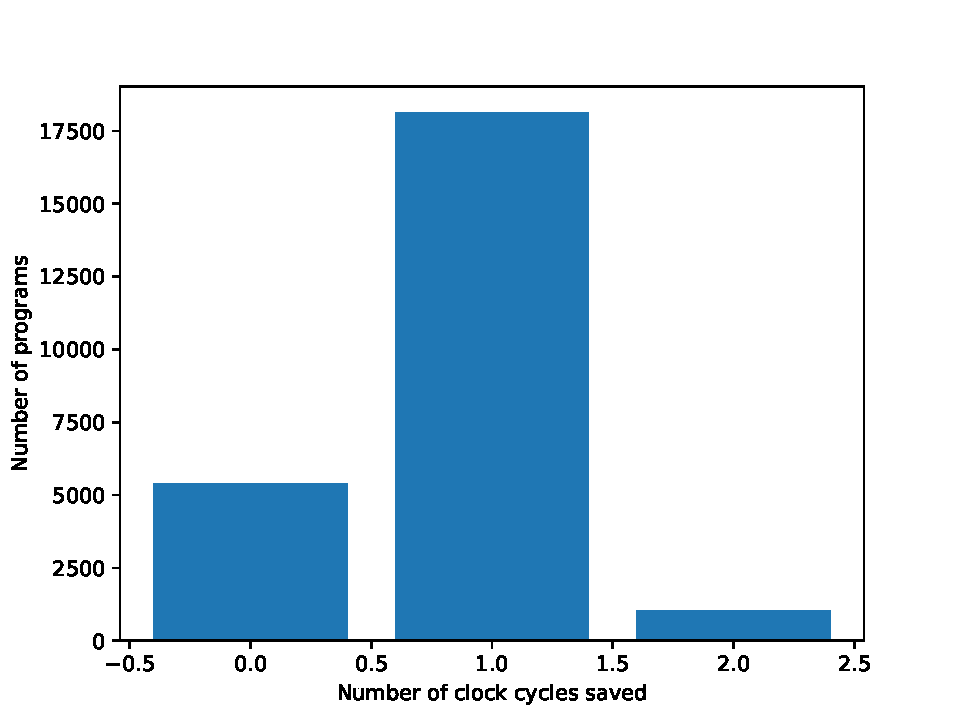
\includegraphics[scale=0.5]{add_count.pdf}
        \caption{Count of programs after merging for the number adders saved.}
        \label{Fig4}
    \end{figure}

    Our testing was done with 6 possible mergings; which interleave program statements. 
    Normally, merging is done by sequentializing a thread after another. 
    But here, merging was performed on a more fine grained level. 
    Is this useful though? Can we do away with just simple thread level merging? 
    Turns out, interleaving forms of merging do help us; more clock cycles as well as more resources can be saved.

    Fig~\ref{Fig5} showcases for each merging strategy, the amount of programs that benefited in saving clock cycles.
    We note that the trend is same, overall around 70percent of the programs benefit by merging; saving clock cycles.
    \begin{figure}
        \centering
        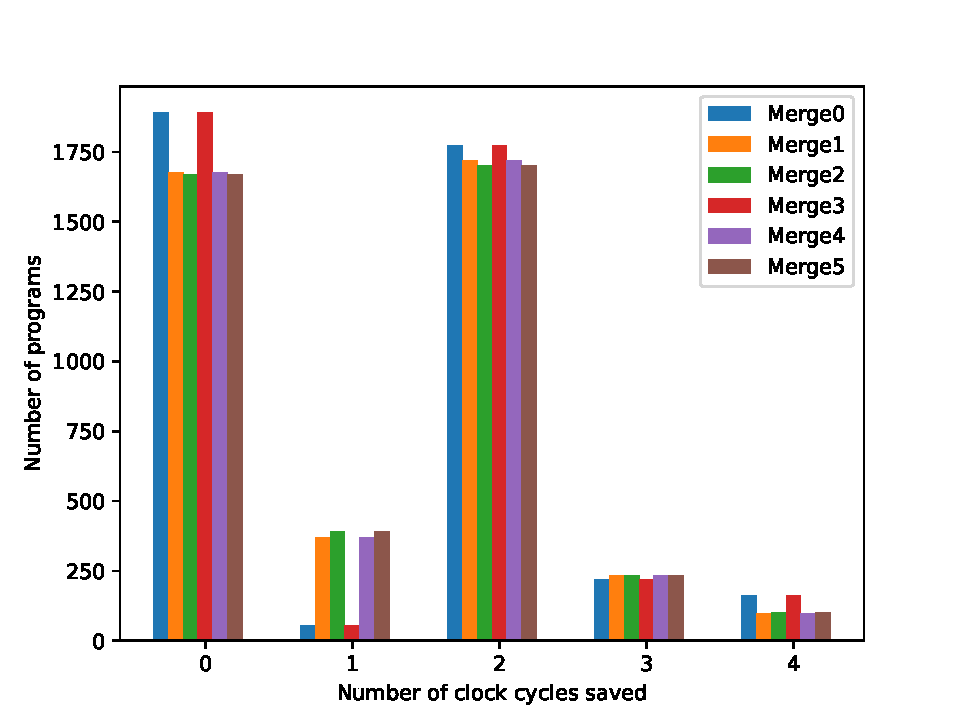
\includegraphics[scale=0.5]{per_merge_clck_saved.pdf}
        \caption{Graph showing for each merging strategy, the number of programs where merging saved clock cycles.}
        \label{Fig5}
    \end{figure}
    
    Fig~\ref{Fig6} showcases for each merging strategy, the amount of programs that benefited in saving adders.
    We once again, note that in most cases, the amount of adders required after merging reduces at least by 1; irrespective of what merging strategy we use. 
    \begin{figure}
        \centering
        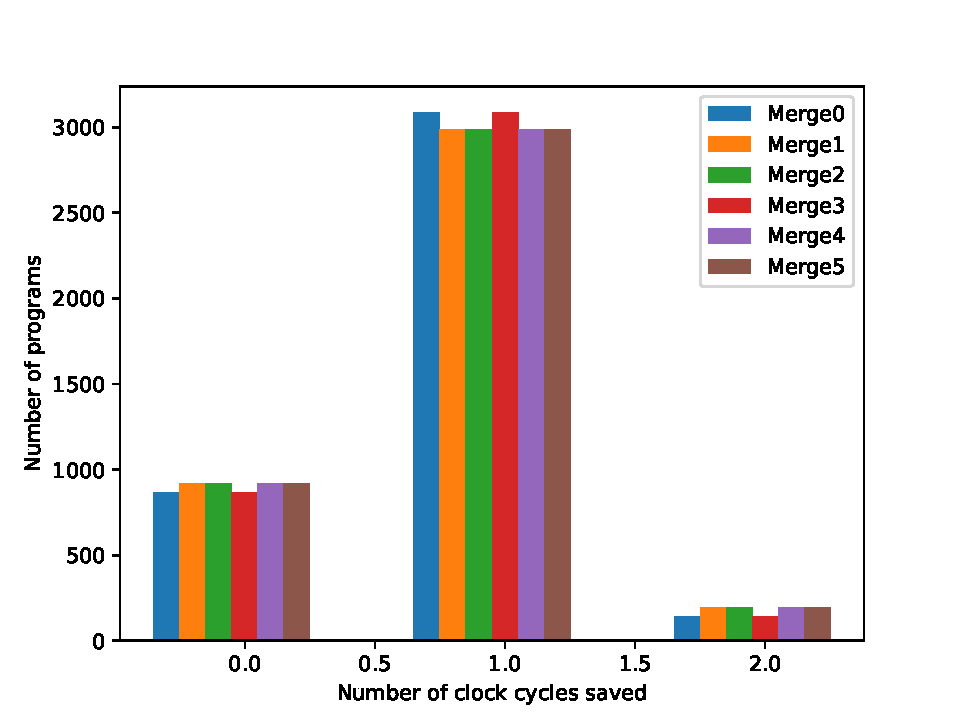
\includegraphics[scale=0.5]{per_merge_add_saved.pdf}
        \caption{Graph showing for each merging strategy, the number of programs where merging saved adders.}
        \label{Fig6}
    \end{figure}

    The above results show us that merging as an optimization is helpful in addressing the resource constraint problem.
    In addition, we do not detriment the overall clock cycles required for the program; this is always bounded by the worst case clock cycles of the original program.
    Moreover, in most cases, we even improve on this bound. 
    
    So far the above statistics does not indicate whether we require all forms of merging. 
    It is important to note that simple merging one thread after the other did not always result in the best resource usage and clock cycles.
    For instance, for the program in Fig~\ref{ex1}, the best merging optimization was interleaving t2's first statement after t1's first statement. Followed by t1's second statement and t2's second statement. 
    \begin{figure}
        \centering
        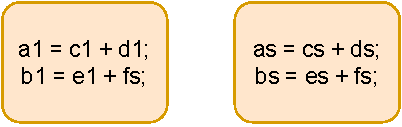
\includegraphics[scale=0.5]{Ex2.pdf}
        \caption{Program for which Merging by interleaving program statements results in a better schedule.}
        \label{ex1}
    \end{figure}

    The schedule for merging this way is given in Fig~\ref{ex1-schd}.
    The blue arrow represnt the memory dependency edges.
    The red circles represent the appropriate clock cycles when an action can be performed; as prescribed by greedy scheduling.
    The green boxes reprsent memory reads and blue boxes memory writes.
    The yellow arrow shows the order in which the two threads were merged.
    The overall schedule saved 2 clock cycles and 1 adder. 
    \begin{figure}
        \centering
        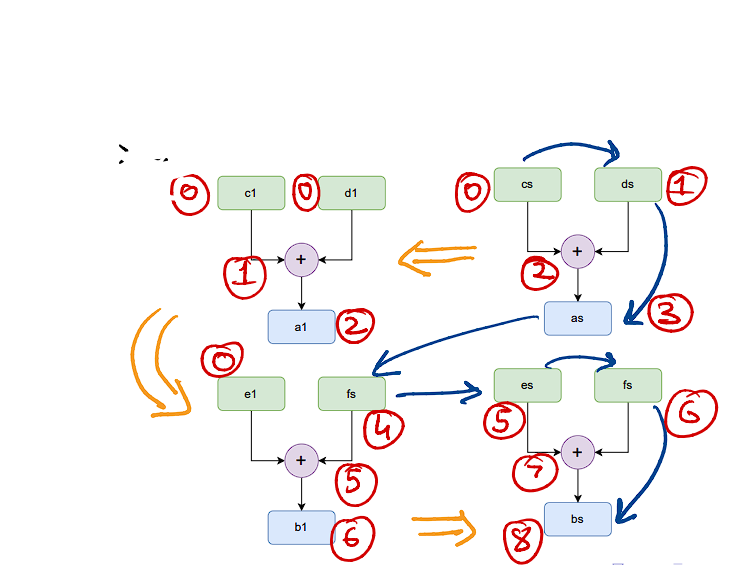
\includegraphics[scale=0.5]{Ex_schd.PNG}
        \caption{The schedule for merging in an interleaved fashion, giving us better schedule in comparison.}
        \label{ex1-schd}
    \end{figure}

    \section{Discussion}

    %Mention limitation as merging is not a safe transformation in many models of concurrency and a debatable feature to include.
    The primary limitation of merging is that this optimization is still not sound for programming languages such as Java and C11. 
    While behavioral models do intend to be written in C-style (for example in LegUp), one would need a different concurrency model to incorporate this optimization.
    The second limitation is the lack of conditionals and loops.
    Incorporating these would make merging at the implementation level more complex, as we would have to consider control flow also and merge parts of another thread only outside conditionals and loops of the primary thread, and so on. 
    Lastly, the scheduling strategy tested for this has only been Greedy.

    %Future work can be done as FPGA synthesis might have different requirements when it comes to memory consistency
    Future work in this line can be done by making merging more fine grained, and interleave at the level of memory accesses, and not program statements. 
    The ideal goal would be to come up with a global analysis that identifies for a given concurrent program, the best merging optimization for sets of threads that save resources as well as clock cycles.
    In addition, it would be nice to see how other optimizations done by HLS tools play in conjuction with merging to give a better synthesized tool. 


    \section{Conclusions}
    %Summarize what was done 
    I tried to address the scheduling problem of fine grained concurrent programs. 
    Previous work have placed no resource constraint while addressing this problem.
    I viewed the resource constraint problem as an optimization that can be done at the behavioral model level before scheduling.
    The optimization helped in addressing the resource constraint problem on most programs considered for benchmarking. 
    It was noted that different variants of the optimization may be required to get least required resources.


    \bibliographystyle{ACM-Reference-Format}
    \bibliography{ref}


\end{document}